% !TEX root = ../report.tex
\chapter{Project Management}\label{pm}

The project was managed throughout by an elected Project Manager (PM) 
(Andrew Fagan), who was tasked with ensuring tasks were 
completed in the timeline decided by the whole group. This 
allowed every member in the group to have an equal voice in 
decisions regarding the project while still having a overall 
manager of the timeline. Using this system, with a minimal 
number of managers and no strictly assigned teams provided
workflow fluidity and flexibility and thus no work was restricted 
to a specific subset of the group. This also improved the 
group's understanding of the project as a whole and the aspects 
which will be detailed herein. 

\section{Project Structure}\label{pm/structure}

It was determined early in the timeline of the project that many members of the 
group were familiar with Agile methodologies\todo{cite}, and were in favour of 
adopting such a methodology into the project structure. Upon review, it was 
decided that this was not fully possible, as iterating many times, particularly on 
mechanical design aspects, would be costly and time consuming. Hence, it was 
decided to adopt Agile concepts where possible. The project was broken into high 
level ``projects'' on GitHub. Within each ``project'', a broad range of high level 
issues were created which team members were able to assign themselves to. If 
issues remained unassigned from the previous group meeting, the PM was tasked with 
assigning at the next. Individual team members assigned to an issue also had the 
responsibility of creating additional dependent issues or linking issues together 
as they felt appropriate, to allow bottlenecks to be identified. These issues can 
be seen as analogous to the backlog of many Agile methodologies. The PM also had 
the responsibility of monitoring timelines on issues and moving team members 
between issues if needed, to spread areas of expertise or solve ``blocking'' 
issues, for example.

Team members working on issues had the freedom to approach them as they felt 
appropriate, which led to some issues such as PCB design and Comms design being 
approached in a highly iterative manner, again in line with Agile methodologies. 
The high level software architecture however remained broadly intact for the 
entirety of the project, as too many other issues relied on this.

Regular meetings were held with the project supervisor to report progress, with no 
more than three weeks between meetings.
	

\subsection{Consultations}\label{pm/consultations}
Throughout the project a number of members of academic staff 
were consulted to obtain an expert's opinion on either 
discussions or decisions made by the group. 
Staff from the EEE, CIS and EMEA departments were 
consulted at various stages in the project, bringing together 
each of the individual components of the robot. 

From the EMEA department, Dr Mark Post (now at York University) 
was consulted in the planning stages of the project. With a 
background in robotic vehicles and SLAM, Dr Post was consulted 
with a view to obtaining as much knowledge as possible 
surrounding the possibilities for operating system to use, 
possible SLAM implementations, potential objectives and 
timescales for parts of the project. Only one meeting took place 
as Dr Post moved to York University shortly after the meeting, 
however, the meeting was highly beneficial and gave a vast 
insight into existing solutions and software, whilst highlighting 
potential pitfalls which could be encountered throughout 
the project.

Dr James Irvine, EEE Department, was consulted informally  
regarding the use of Sockets for communication using a Wireless 
Ad-hoc Network (WANET). Dr Irvine was approached with an 
assumption that using the Python Socket library to send 
serialised data between the Raspberry Pis would be a robust 
method of communication between the robots. This was confirmed 
by Dr Irvine with the additional suggestion to serialise the data
as JSON objects. 


Dr Gordon Dobie, EEE Department, was consulted towards the end 
of the project regarding the tuning of the PID controller. 
Members of the group met with Dr Dobie and explained the PID tuning 
processes undertook to that point. He explained that although 
PID was conceptually useful, a more simple PD rate control system 
\ref{litreview/control/ratecontrol} would be more appropriate 
in this particular case. Following the in-depth investigations made 
into PID controllers, the group was fairly confident following some 
basic guidance, provided by Dr Dobie, on implementing the 
recommended system. 

Prior to the arrangement of the meeting with Dr Dobie, Dr Phil 
Rogers was consulted regarding the tuning of the PID controller. 
He suggested providing a frame of reference in order to correct 
the PID controller and maintain a straight line with regards to 
its reference frame. While the group waited on the meeting with 
Dr Dobie, a specialist in PID control, Dr Rogers advice was 
followed and SLAM was progressed in the interim.   

\subsection{Mechanical Workshop}\label{pm/mechshop}
The construction of the modular maze used for testing \ref{mech/
maze} was outsourced to the mechanical workshop located in the 
EEE department at the university. A number of discussions with 
the mechanical workshop were used to specify the design  
before and during construction. The design was iterated upon multiple times to achieve the best 
possible outcome. More information can be found in Section~\ref{test/maze}.  

\section{Timeline}\label{pm/timeline}
The Gantt chart shown here in Figure~\ref{figure:gantt} was created 
using the objectives and their respective sub-objectives (Section~
\ref{introduction/objectives}). The timescales were determined 
approximately using knowledge obtained from research and 
consultations, with additional time added to account for possible 
technical risks. In line with the agile methodology adopted, the tasks 
were given appropriate time and a small margin for error within the 
Gantt chart. For example, assembly of remaining robots was 
allocated a longer time than expected as this involved lead times 
for components and also spanned the period of time when the labs 
were closed and construction work was not possible.

Figure~\ref{figure:gantt} shows a Gantt chart of the project timeline.


\begin{landscape} % Rotates the image on the page
\global\pdfpageattr\expandafter{\the\pdfpageattr/Rotate 90} % Rotates the page in the PDF output
\begin{figure}[!p]\centering
    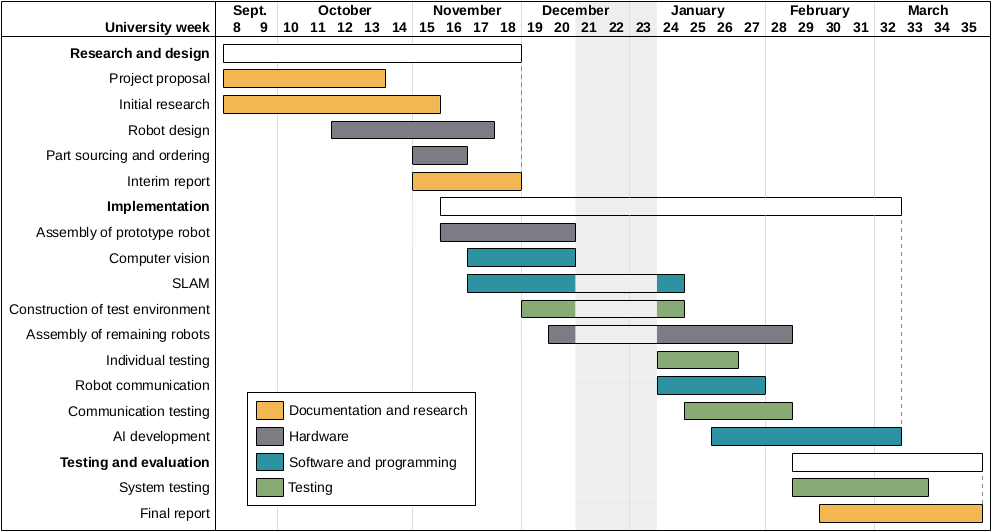
\includegraphics[width=1\linewidth]{gantt}
    \caption{Gantt chart}\label{figure:gantt}
\end{figure}
\end{landscape}
\global\pdfpageattr\expandafter{\the\pdfpageattr/Rotate 0}

The Gantt chart was adhered to for the most part in the early to 
mid stages of the project. Towards the latter stages of the 
project slippage occurred in the timelines which meant that some 
of the later objectives were not completed fully. A number 
of the slippages in the latter stages were due to unforeseeable 
electrical or mechanical issues. Multiple issues arose and had to 
be handled in the latter stages of the project including motors 
leaking grease, standard AA batteries being drained at an 
excessive rate and one Raspberry Pi being shorted and killed 
during the testing phase. Several technical slippages occurred in the Gantt 
chart in the latter stages namely: PID tuning (see Section~\ref{soft/PID}) and SLAM, which was eventually spilt into 2 parts (see Sections~\ref{soft/odometry} \& ~\ref{soft/SLAM}).

\section{Risk Evaluation}\label{pm/riskeval}
A risk evaluation took place at the beginning of the project and 
was re-evaluated at the time of the interim report. The technical 
risks evaluated at this time mainly centred on the possible lead 
times for ordering parts. At the time of ordering, this was 
thought to be a major issue, and so one part for each of the three 
robots was ordered at this time. One part of the order in 
particular was not in stock and was back-ordered with an expected 
lead-time of 5 weeks from the end of December. This happened to 
not be the case and ordering lead times were not an issue within 
the project on the whole as other work, such as designing and 
constructing the modular maze for testing could be carried out in 
the interim. 

It was then expected that component failure would form the second 
main technical risk of the project. This was partly true, as 
mentioned in Section~\ref{pm/timeline}, as a number of components 
failed throughout the project and had to either be replaced or 
fixed, consuming time in the project. This was partly mitigated by 
the time left at the end of the project, however, the replacement 
of these parts did impact on system testing time, as the 
integration testing for each of the replacement components had to 
be repeated. 


